\documentclass[10pt,a4paper]{amsart}
\usepackage[margin=19mm]{geometry}
\usepackage{amsmath,amssymb,mathtools}
\usepackage[scr=rsfs,cal=euler]{mathalfa}
\usepackage{xfrac}
\usepackage[unicode,hidelinks,bookmarks=false]{hyperref}
\newcommand{\ie}{i.e.\ }
\newcommand{\cf}{cf.\ }
\newcommand{\resp}{respectively\ }
\newcommand{\Subsection}{\subsection}
\providecommand{\nobreakdash}{\nobreak\hbox{-}}
\setlength{\emergencystretch}{2em}
\multlinegap0pt
\usepackage{tikz}
\newtheorem{theorem}{Theorem}[section]
\newtheorem{lemma}[theorem]{Lemma}
\newtheorem{cor}[theorem]{Corollary}
\newtheorem{definition}[theorem]{Definition}
\newtheorem{example}[theorem]{Example}
\newtheorem{xca}[theorem]{Exercise}
\newtheorem{remark}[theorem]{Remark}
\numberwithin{equation}{section}
\begin{document}
\title[Sharp Bounds for Kulli-Basava Indices of Graphs]{Sharp Bounds for Kulli-Basava Indices of Graphs}
\author{Sanju Vaidya, Jeff Chang}
\date{}
\maketitle
\noindent\emph{Source and licence.} Sharp Bounds for Kulli-Basava Indices of Graphs. Version arXiv:2609.28143v1 (CC BY 4.0). This material is distributed under the Creative Commons Attribution 4.0 International licence, http://creativecommons.org/licenses/by/4.0/, as recorded in the arXiv OAI licence metadata for this exact version and shown on the abstract page https://arxiv.org/abs/2609.28143v1. Full rights notice: licenses/arxiv-2609.28143-CC-BY-4.0.txt.\par\smallskip
\noindent\textit{Editorial scope.} Counted unit: the original \texttt{theorem} environment \texttt{Theorem3} at source lines 379--408 together with its complete proof at lines 410--424; the delivered document keeps source lines 97--425 so that every referenced label and every citation resolves inside it. Native editable source is the paper's own concatenated TeX; the AMS wrapper is editorial formatting only. No publisher class, upstream script or unrelated artwork is redistributed.\par\smallskip\noindent\textit{Reference note.} This article ships no compiled bibliography (biblatex); the entries delivered here are composed from the author's own BibTeX (.bib) fields, with no field invented and no entry dropped.
\begin{theorem}[Jensen's inequality]\label{Jensen}
For any positive integer $k$, if $f$ is strictly convex (that is, $f''(x)>0$), then
\[
f\left(\frac{1}{k}\sum_{i=1}^{k}x_i\right)\leq \frac{1}{k}\sum_{i=1}^{k}f(x_i),
\]
with equality if and only if $x_1=x_2=\cdots=x_k$. If $-f$ is strictly convex, then the inequality is reversed.
\end{theorem}


We also use the following result of Zhou \cite{zhou2006note} for triangle- and quadrangle-free graphs.

\begin{theorem}
Let $G$ be a triangle- and quadrangle-free graph with $n$ vertices. Then its first Zagreb index satisfies $M_1\leq n(n-1)$.
\end{theorem}

We also use the following lower bound of Filipovski \cite{filipovski2021new} for the first Zagreb index of a graph with a prescribed clique number. Recall that the clique number of a graph $G$ is the order of a largest complete subgraph of $G$.

\begin{theorem} Let $G$ be a graph with $n$ vertices, $m$ edges, and clique number $w$. Then
\[
M_1\geq 4mn+\frac{n^3}{w^2}-n^3,
\]
with equality if and only if $G$ is a regular graph of degree $k$ and $w=\frac{n}{n-k}$.
\end{theorem}

\section{Formulas and Bounds for Kulli-Basava Indices}

In this section, we establish formulas for the general Kulli-Basava index and use them to derive sharp upper and lower bounds. We first recall the following lemma, proved by Vaidya and Chang \cite{vaidya2024sharp}.

\begin{lemma}\label{Lemma}
Let $p$ and $q$ be positive integers such that $p<q$, and let $\alpha\in\mathbb{R}\setminus\{0,1\}$. Then the following statements hold.
\begin{enumerate}
\item If $\alpha<0$ or $\alpha>1$, then $(p+i)^\alpha-p^\alpha-i\left(\frac{q^\alpha-p^\alpha}{q-p}\right)\leq 0$ for $1\leq i\leq q-p-1$. If $0<\alpha<1$, then the inequality is reversed.

\item If $\alpha<0$ or $\alpha>1$, then $(p+i)^\alpha-p^\alpha-i((p+1)^\alpha-p^\alpha)\geq 0$ for $2\leq i\leq q-p$. If $0<\alpha<1$, then the inequality is reversed.

\end{enumerate}
\end{lemma}

We also need the following lemma.

\begin{lemma}\label{Lemma2}
Let $p$ and $q$ be positive integers such that $p<q$. Then the following statements hold.
\begin{enumerate}
\item $\ln(p+i)-\ln(p)-i\left(\frac{\ln(q)-\ln(p)}{q-p}\right)\geq 0$ for $1\leq i\leq q-p-1$.

\item $\ln(p+i)-\ln(p)-i(\ln(p+1)-\ln(p))\leq 0$ for $2\leq i\leq q-p$.

\end{enumerate}
\end{lemma}
\begin{proof}
The results follow from the fact that the function $f(x)=\frac{\ln(x)-\ln(p)}{x-p}$ is decreasing for $x>p$.
\end{proof}

\begin{theorem}\label{Theorem1}
Let $G$ be a graph with $n\geq 3$ vertices and $m$ edges. Let $n_i$ denote the number of vertices with edge neighborhood degree $i$, and let $\delta$ and $\Delta$ denote the minimum and maximum edge neighborhood degrees, respectively, where $\delta\neq\Delta$. Let $a\in\mathbb{R}\setminus\{0,1\}$ and set $s_a=\frac{\Delta^a-\delta^a}{\Delta-\delta}$. Then the following statements hold.
    \begin{enumerate}
\item 
        \[KB^a(G) = n\delta^a +  (2M_1 - 4m - n\delta)s_a +\sum_{i =1}^{\Delta - \delta - 1}n_{\delta + i} \left[(\delta + i)^a - \delta^a  - is_a\right].\]

If $a<0$ or $a>1$, the coefficients $(\delta+i)^a-\delta^a-is_a$ are nonpositive for $1\leq i\leq\Delta-\delta-1$; if $0<a<1$, they are nonnegative.

\item If $a>1$, then the natural logarithm of the general multiplicative Kulli-Basava index is
\[
\begin{aligned}
\ln\left[\prod_{v\in V(G)}S_e(v)^a\right]
&=a\left[n\ln(\delta)+\frac{(2M_1-4m-n\delta)(\ln\Delta-\ln\delta)}{\Delta-\delta}\right.\\
&\qquad\left.+\sum_{i=1}^{\Delta-\delta-1}n_{\delta+i}\left(\ln(\delta+i)-\ln(\delta)-i\frac{\ln\Delta-\ln\delta}{\Delta-\delta}\right)\right].
\end{aligned}
\]
Moreover, the coefficients of $n_{\delta+i}$ are nonnegative for $1\leq i\leq\Delta-\delta-1$.
\end{enumerate} 
\end{theorem}
\begin{proof}

By part (iii) of Lemma 2.2 in \cite{basavanagoud2019kulli}, $\sum_{i=\delta}^\Delta i n_i=2M_1-4m$. We also have $n=\sum_{i=\delta}^\Delta n_i$. Solving these equations for $n_\Delta$ gives
\[
n_\Delta=\frac{2M_1 - 4m - n\delta - \sum_{i=\delta + 1}^{\Delta  - 1}(i - \delta)n_i}{\Delta - \delta}.
\]

Writing $KB^a(G)$ in terms of $n_i$ for $\delta\leq i\leq\Delta$ and substituting $n_\delta=n-\sum_{i=\delta+1}^\Delta n_i$, we obtain
\[
KB^a(G) = \sum_{i=\delta}^\Delta  i^a n_i = \delta^a\left( n - \sum_{i= \delta + 1}^\Delta n_i\right) + \sum_{i=\delta + 1}^\Delta  i^a n_i = n\delta^a + \sum_{i = \delta + 1}^\Delta  n_i(i^a - \delta^a).
\]
Substituting the expression for $n_\Delta$ into this sum and applying Lemma \ref{Lemma} yields part (1).

For part (2), write the natural logarithm of the general multiplicative Kulli-Basava index in terms of $n_i$, $\delta\leq i\leq\Delta$, and substitute $n_\delta=n-\sum_{i=\delta+1}^\Delta n_i$. This gives
\[
\ln\left[\prod_{v\in V(G)}S_e(v)^a\right]=a\sum_{i=\delta}^\Delta \ln(i)n_i=a\left[n\ln(\delta)+\sum_{i=\delta+1}^\Delta n_i(\ln(i)-\ln(\delta))\right].
\]
Substituting $n_\Delta$ into the sum and applying part (1) of Lemma \ref{Lemma2} completes the proof.

\end{proof}

The following corollary gives upper and lower bounds for the general Kulli-Basava index, depending on the value of $a$. All the bounds are sharp.

\begin{cor}\label{Cor1}
Let $G$ be a graph with $n\geq 3$ vertices and $m$ edges. Let $\delta$ and $\Delta$ denote the minimum and maximum edge neighborhood degrees, respectively, where $\delta\neq\Delta$. Let $a\in\mathbb{R}\setminus\{0,1\}$ and set $s_a=\frac{\Delta^a-\delta^a}{\Delta-\delta}$. Then the following statements hold.

\begin{enumerate}
        \item If $a < 0$ or $a > 1$, the upper bound for the general Kulli-Basava index is $ KB^a(G) \leq n\delta^a +  (2M_1 - 4m - n\delta)s_a$.

    
    \item If $0<a<1$, the corresponding lower bound is $KB^a(G)\geq n\delta^a+(2M_1-4m-n\delta)s_a$.

    \item If $a>1$, then the lower bound for the natural logarithm of the general multiplicative Kulli-Basava index is 
$\ln\left[\prod_{v\in V(G)}S_e(v)^a\right]\geq a\left[n\ln(\delta)+\frac{(2M_1-4m-n\delta)(\ln\Delta-\ln\delta)}{\Delta-\delta}\right]$.
    

\end{enumerate}
In all three parts, equality holds for any graph whose vertices have edge neighborhood degree $\delta$ or $\Delta$.
\end{cor}

\begin{proof}
The results follow from Theorem \ref{Theorem1}.
\end{proof}

\begin{example}
For the graph in Figure \ref{fig:1}, $\delta=3$, $\Delta=18$, $m=n=12$, and $M_1=72$. Every vertex has edge neighborhood degree $3$ or $18$, so the graph attains the bounds in parts (1)--(3) of Corollary \ref{Cor1}.
\begin{figure}[h]
\centering
\begin{minipage}{.4\textwidth}
  \centering
  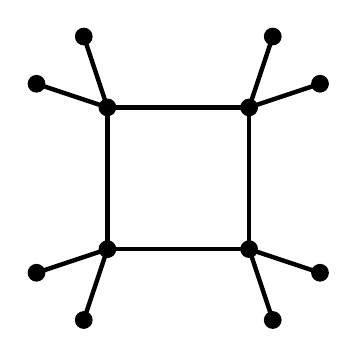
\begin{tikzpicture}[scale=0.3]
\draw[ultra thick] (-3,3) -- (3,3) -- (3,-3)--(-3,-3) -- (-3,3);
\draw[ultra thick] (3,3)--(6,4);
\draw[ultra thick] (3,3)--(4,6);
\draw[ultra thick] (-3,3)--(-4,6);
\draw[ultra thick] (-3,3)--(-6,4);
\draw[ultra thick] (3,-3)--(6,-4);
\draw[ultra thick] (3,-3)--(4,-6);
\draw[ultra thick] (-3,-3)--(-6,-4);
\draw[ultra thick] (-3,-3)--(-4,-6);
\filldraw[black] (3,3) circle (10pt);
\filldraw[black] (-3,3) circle (10pt);
\filldraw[black] (3,-3) circle (10pt);
\filldraw[black] (-3,-3) circle (10pt);
\filldraw[black] (6,4) circle (10pt);
\filldraw[black] (4,6) circle (10pt);
\filldraw[black] (-6,4) circle (10pt);
\filldraw[black] (-4,6) circle (10pt);
\filldraw[black] (6,-4) circle (10pt);
\filldraw[black] (4,-6) circle (10pt);
\filldraw[black] (-6,-4) circle (10pt);
\filldraw[black] (-4,-6) circle (10pt);
\end{tikzpicture}
\caption{A graph attaining the bounds in Corollary \ref{Cor1}.}
  \label{fig:1}
\end{minipage}%

\end{figure}
\end{example}

The following corollary gives a sharp upper bound for the Kulli-Basava index of triangle- and quadrangle-free graphs. The bound depends on the numbers of vertices and edges and on the minimum and maximum edge neighborhood degrees.

\begin{cor}
Let $G$ be a triangle- and quadrangle-free graph with $n\geq 3$ vertices and $m$ edges. Let $\delta$ and $\Delta$ denote the minimum and maximum edge neighborhood degrees, respectively, where $\delta\neq\Delta$. Let $a>1$ and set $s_a=\frac{\Delta^a-\delta^a}{\Delta-\delta}$. Then
\[
KB^a(G)\leq n\delta^a+(2n(n-1)-4m-n\delta)s_a,
\]
with equality for a star graph.
\end{cor}

\begin{proof}
Zhou \cite{zhou2006note} proved that the first Zagreb index of a triangle- and quadrangle-free graph satisfies $M_1\leq n(n-1)$. Combining this inequality with Theorem \ref{Theorem1} gives the result.
\end{proof}

The following theorem provides additional formulas for the general and general multiplicative Kulli-Basava indices.


\begin{theorem}\label{Theorem2}
Let $G$ be a graph with $n\geq 3$ vertices and $m$ edges. Let $n_i$ denote the number of vertices with edge neighborhood degree $i$, and let $\delta$ and $\Delta$ denote the minimum and maximum edge neighborhood degrees, respectively. Let $a\in\mathbb{R}\setminus\{0,1\}$. Then the following statements hold.
 \begin{enumerate}
 \item
\begin{align*}
KB^a(G)={}&n\delta^a+(2M_1-4m-n\delta)\bigl((\delta+1)^a-\delta^a\bigr)\\
&+\sum_{i=2}^{\Delta-\delta}n_{\delta+i}
\left[(\delta+i)^a-\delta^a-i\bigl((\delta+1)^a-\delta^a\bigr)\right].
\end{align*}
   
If $a<0$ or $a>1$, the coefficients $(\delta+i)^a-\delta^a-i((\delta+1)^a-\delta^a)$ are nonnegative for $2\leq i\leq\Delta-\delta$; if $0<a<1$, they are nonpositive.

\item If $a>1$, then the natural logarithm of the general multiplicative Kulli-Basava index is
\[
\begin{aligned}
\ln\left[\prod_{v\in V(G)}S_e(v)^a\right]
&=a\left[n\ln(\delta)+(2M_1-4m-n\delta)(\ln(\delta+1)-\ln\delta)\right.\\
&\qquad\left.+\sum_{i=2}^{\Delta-\delta}n_{\delta+i}\left(\ln(\delta+i)-\ln(\delta)-i(\ln(\delta+1)-\ln\delta)\right)\right].
\end{aligned}
\]
Moreover, the coefficients of $n_{\delta+i}$ are nonpositive for $2\leq i\leq\Delta-\delta$.
\end{enumerate} 
 
\end{theorem}

\begin{proof}

By part (iii) of Lemma 2.2 in \cite{basavanagoud2019kulli}, $\sum_{i=\delta}^\Delta i n_i=2M_1-4m$. We also have $n=\sum_{i=\delta}^\Delta n_i$. Hence $n_\delta+n_{\delta+1}=n-\sum_{i=\delta+2}^\Delta n_i$ and $\delta n_\delta+(\delta+1)n_{\delta+1}=2M_1-4m-\sum_{i=\delta+2}^\Delta i n_i$. Solving for $n_\delta$ and $n_{\delta+1}$, substituting the results into $KB^a(G)=\sum_{i=\delta}^\Delta i^a n_i$, and applying Lemma \ref{Lemma} proves part (1). For part (2), write the natural logarithm of the general multiplicative Kulli-Basava index in terms of $n_i$ and substitute $n_\delta=n-\sum_{i=\delta+1}^\Delta n_i$. Then
\[
\ln\left[\prod_{v\in V(G)}S_e(v)^a\right]=a\sum_{i=\delta}^\Delta\ln(i)n_i=a\left[n\ln(\delta)+\sum_{i=\delta+1}^\Delta n_i(\ln(i)-\ln(\delta))\right].
\]
Substituting $n_{\delta+1}$ into the sum and applying part (2) of Lemma \ref{Lemma2} completes the proof.

\end{proof}

The following corollary gives sharp bounds for the general and general multiplicative Kulli-Basava indices, depending on the value of $a$.

\begin{cor}
Let $G$ be a graph with $n\geq 3$ vertices and $m$ edges. Let $\delta$ denote the minimum edge neighborhood degree, and let $a\in\mathbb{R}\setminus\{0,1\}$. Then the following statements hold.

\begin{enumerate}
       
\item If $a < 0$ or $ a > 1$, then the lower bound for the general Kulli-Basava index is $KB^a(G) \geq n\delta^a +  (2M_1 - 4m - n\delta) ((\delta + 1)^a - \delta^a)$.

\item If $0 < a < 1$, then the upper bound for the general Kulli-Basava index is $KB^a(G)  \leq n\delta^a +  (2M_1 - 4m - n\delta) ((\delta + 1)^a - \delta^a)$.

\item If $a>1$, then
\[
\ln\left[\prod_{v\in V(G)}S_e(v)^a\right]\leq a\left[n\ln(\delta)+(2M_1-4m-n\delta)(\ln(\delta+1)-\ln\delta)\right].
\]

   
In all three parts, equality holds for every regular graph.
    
\end{enumerate}
       
\end{cor}
\begin{proof}
The results follow from Theorem \ref{Theorem2}.
\end{proof}


The following corollary gives a sharp lower bound for graphs with a prescribed clique number.

\begin{cor}
Let $G$ be a graph with $n\geq 3$ vertices, $m$ edges, and clique number $w$. Let $\delta$ denote the minimum edge neighborhood degree, and let $a>1$. Then
\[
KB^a(G)\geq n\delta^a+\left(4m(2n-1)+2n^3\left(\frac{1}{w^2}-1\right)-n\delta\right)((\delta+1)^a-\delta^a),
\]
with equality if $G$ is regular of degree $k$ and $w=\frac{n}{n-k}$.
\end{cor}
\begin{proof}
The result follows from Theorem \ref{Theorem2} and Theorem 2.8 of Filipovski \cite{filipovski2021new}.
\end{proof}

The following theorem gives further bounds for the general Kulli-Basava index.

\begin{theorem}
Let $G$ be a graph with $n\geq 3$ vertices and $m$ edges, and let $a\in\mathbb{R}\setminus\{0,1\}$.

\begin{enumerate}
       
\item If $a < 0$ or $a > 1$, then the lower bound for the general Kulli-Basava index is $KB^a(G) \geq n^{1 - a} (2M_1 - 4m)^a $.

\item If $0<a<1$, then the upper bound  is $KB^a(G)  \leq n^{1 - a}(2M_1 - 4m)^a$.
   

    
\end{enumerate}
In both parts, equality holds if $S_e(v)$ is the same for every vertex $v$.
\end{theorem}
\begin{proof}
For part (1), assume that $a<0$ or $a>1$ and let $f(x)=x^a$ for $x>0$. Since $f''(x)>0$, the function is strictly convex. Applying Jensen's inequality (Theorem \ref{Jensen}) to the edge neighborhood degrees and simplifying proves the bound.

For part (2), if $0<a<1$, then $-f(x)=-x^a$ is strictly convex. Applying Jensen's inequality yields the upper bound. Equality holds in both cases when $S_e(v)$ is constant over all vertices $v\in V(G)$.
\end{proof}

The following corollary gives a sharp upper bound for the Kulli-Basava index of triangle-free graphs. The bound depends on the numbers of vertices and edges and on the minimum and maximum vertex degrees.

\begin{cor}
Let $G$ be a triangle-free graph with $n\geq 3$ vertices and $m$ edges. Let $d$ and $D$ denote the minimum and maximum vertex degrees, respectively, where $d\neq D$, and let $a>1$. Then
\[
KB^a(G)\leq(n-2)^a\left[nd^a+(2m-nd)\left(\frac{D^a-d^a}{D-d}\right)\right],
\]
with equality for a star graph.
\end{cor}

\begin{proof}
Because $G$ is triangle-free, every edge $uv\in E(G)$ satisfies $d(u)+d(v)\leq n$. Therefore, the edge neighborhood degree of any vertex $v$ satisfies $S_e(v)\leq(n-2)d(v)$. Hence $KB^a(G)\leq(n-2)^aM_1^a(G)$. Vaidya and Chang \cite{vaidya2024sharp} proved that $M_1^a\leq nd^a+(2m-nd)\left(\frac{D^a-d^a}{D-d}\right)$, and the result follows.
\end{proof}

In Theorem 2.2, Hu, Li, Shi, Xu, and Gutman \cite{hu2005molecular} established formulas for the maximum and minimum zeroth-order general Randi\'{c} indices of $(n,m)$ molecular graphs when $2m-n$ is congruent to $0$, $1$, or $2$ modulo $3$ and the maximum vertex degree is $4$. The following theorem extends this approach and gives sharp bounds for the general Kulli-Basava index when $2M_1-4m-n\delta$ is congruent to an arbitrary integer $r$ modulo $\Delta-\delta$, where $0\leq r<\Delta-\delta$, and the maximum edge neighborhood degree is at least $3$.


\begin{theorem}\label{Theorem3}
Let $G$ be a graph with $n\geq 3$ vertices and $m$ edges. Let $n_i$ denote the number of vertices with edge neighborhood degree $i$, and let $\delta$ and $\Delta$ denote the minimum and maximum edge neighborhood degrees, respectively. Assume that $\Delta-\delta\geq2$ and $2M_1-4m-n\delta=q(\Delta-\delta)+r$, where $q$ is a positive integer and $r$ is an integer such that $0\leq r\leq\Delta-\delta-1$. Let $a\in\mathbb{R}\setminus\{0,1\}$ and set $s_a=\frac{\Delta^a-\delta^a}{\Delta-\delta}$. Then the following statements hold.

 \begin{enumerate}
\item If $r=0$ and $n_\Delta=q$, then $G$ is a bi-edge-neighborhood-degree graph whose vertices have edge neighborhood degrees $\delta$ and $\Delta$.

  \item If $r \geq 1$ and $n_{\Delta} = q$, then $n_i = 0$ for $\delta + r + 1 \leq i \leq \Delta  - 1$ and $n_{\delta + r} \leq 1$.

\item If $r\geq1$, either $a<0$ or $a>1$, and $n_{\delta+r}\neq0$, then
\[
KB^a(G)\leq n\delta^a+(2M_1-4m-n\delta)s_a+(\delta+r)^a-\delta^a-rs_a.
\]

\item If $r\geq1$, $0<a<1$, and $n_{\delta+r}\neq0$, then
\[
KB^a(G)\geq n\delta^a+(2M_1-4m-n\delta)s_a+(\delta+r)^a-\delta^a-rs_a.
\]

\item If $r\geq1$, $a>1$, and $n_{\delta+r}\neq0$, then
\[
\begin{aligned}
\ln\left[\prod_{v\in V(G)}S_e(v)^a\right]\geq
&a\left[n\ln(\delta)+\frac{(2M_1-4m-n\delta)(\ln\Delta-\ln\delta)}{\Delta-\delta}\right.\\
&\qquad\left.+\ln(\delta+r)-\ln(\delta)-r\frac{\ln\Delta-\ln\delta}{\Delta-\delta}\right].
\end{aligned}
\]
 \end{enumerate}
In parts (3)--(5), equality holds if $G$ has $q$ vertices of edge neighborhood degree $\Delta$, one vertex of edge neighborhood degree $\delta+r$, and $n-q-1$ vertices of edge neighborhood degree $\delta$.
 
\end{theorem}

\begin{proof}
By part (iii) of Lemma 2.2 in \cite{basavanagoud2019kulli}, $\sum_{i=\delta}^\Delta i n_i=2M_1-4m$. We also have $n=\sum_{i=\delta}^\Delta n_i$. Solving these equations gives
\[
\sum_{i=\delta+1}^\Delta(i-\delta)n_i=2M_1-4m-n\delta=q(\Delta-\delta)+r.
\]
If $r=0$ and $n_\Delta=q$, then $n_i=0$ for $\delta+1\leq i\leq\Delta-1$, which proves part (1). If $r\geq1$ and $n_\Delta=q$, then $n_i=0$ for $\delta+r+1\leq i\leq\Delta-1$ and $n_{\delta+r}\leq1$, which proves part (2). For part (3), let $r\geq1$ and $n_{\delta+r}\neq0$. By part (1) of Theorem \ref{Theorem1},
$KB^a(G)=n\delta^a +  (2M_1 - 4m - n\delta)s_a +\sum_{i =1}^{\Delta - \delta - 1}n_{\delta + i} \left[(\delta + i)^a - \delta^a  - is_a\right].$

If $a<0$ or $a>1$, then $(\delta+i)^a-\delta^a-is_a\leq0$ for $1\leq i\leq\Delta-\delta-1$. Therefore,

$KB^a(G) \leq n\delta^a +  (2M_1 - 4m -n\delta)s_a + n_{\delta + r} \left[(\delta + r)^a - \delta^a  - (r)s_a\right].$

Since $n_{\delta+r}\neq0$, part (3) follows. Similarly, part (4) follows because $(\delta+i)^a-\delta^a-is_a\geq0$ for $0<a<1$ and $1\leq i\leq\Delta-\delta-1$. Part (5) follows from part (2) of Theorem \ref{Theorem1}. The equality condition in parts (3)--(5) also follows from Theorem \ref{Theorem1}.

\end{proof}

\begin{thebibliography}{99}
\bibitem[]{basavanagoud2019kulli} Basavanagoud, B; Jakkannavar, Praveen. Kulli-Basava indices of graphs. International Journal of Applied Engineering Research 14 (2019) 325--342
\bibitem[]{filipovski2021new} Filipovski, Slobodan. New bounds for the first Zagreb index. MATCH Commun. Math. Comput. Chem 85 (2021) 303--312
\bibitem[]{hu2005molecular} Hu, Yumei; Li, Xueliang; Shi, Yongtang; Xu, Tianyi; Gutman, Ivan. On molecular graphs with smallest and greatest zeroth-order general Randic index. MATCH Commun. Math. Comput. Chem 54 (2005) 425--434
\bibitem[]{vaidya2024sharp} Vaidya, Sanju; Chang, Jeff. Sharp Bounds for Generalized Zagreb Indices of Graphs. arXiv preprint arXiv:2409.06081 (2024)
\bibitem[]{zhou2006note} Zhou, Bo; Stevanovic, Dragan. A note on Zagreb indices. MATCH Commun. Math. Comput. Chem 56 (2006) 571--578
\end{thebibliography}
\end{document}
